\label{sec:2d}
\subsection{Implementation}
The non-parametric estimation was implemented first for the 2 case.  A 2D Gaussian matrix was created, using the specified variance of $\sigma^2=400$ over a range of x-values from -60 to 60.  Similar to the previous lab, class structure was used to streamline the code.  Each of the data clusters, al, bl, cl, were passed into the function TwoD, where the mean and covariance were estimated.  The provided parzen methods, included as part of the OneD class, was then called to estimate the PDF of each of the clusters, using the previously defined 2D Gaussian matrix and and resolution.  The returned parameters p, x, and y were assigned to ap, ax, and ay for Cluster A, bp, bx, and by for Cluster B and so on.  These estimated PDFs for each cluster (ap, bp, cp) were then passed into the ML function to form the classification boundaries.  The ML function steps through each sqare on the grid defined by the resolution, looking for the cluster with the highest probability each time.  A value of 0 is assigned to all elements of the grid ML for which Class A had a higher estimated probability, a value 1 for elements in which Class B was most likely, and a value 2 for elements in which Class C was most likely.  The ML boundaries were then plotted using a contour plot.  

The parametric estimation was implemented to mimic the inputs and outputs of the parzen function in order to simplify the code.  The parametric methods of the TwoD class was then called to estimate the PDF of the cluster.  It used the previously defined resolution as well as the estimated mean and covariance parameters from earlier.  a matrix, p, of probability densities was the result, along with x and y bounds matching the parzen method.  These values, p, x, and y were then passed into the ML method, in the exact same manner as with the non-parametric case and the resulting ML boundaries were plotted using a contour plot.  

\subsection{Results}
For the two dimensional case, there are three clusters of data, all with
different shapes. Parametric estimation was performed, assuming that each
cluster was Gaussian distributed.  The mean and variance were learned from the
data and the resulting classification boundaries were plotted.  These
parametric boundaries do a reasonable job of differentiating the classes from
each other.  For example, the majority of Class A data points will indeed be
classified as A.  The classification boundaries themselves, however, do not
track the boundaries of the classes particularly well. The classification
boundary for Class C (represented by red stars), for example, appears to be
shifted up and to the left of where we would intuitively like it to be.  The
boundary has not physically been shifted anywhere of course, but rather this
apparent "shift" is due to the fact that the classes are not truly Gaussian in
shape.  The classification boundaries are based on statistics that match an
assumed Gaussian model.  The effects of assuming the shape of the PDF can be
further seen by examining the classification boundary between Class A and B
(red + and blue diamond).  Class B is somewhat crescent-shaped, enveloping a
large portion of Class A.  The ML classification boundary, based on estimated
Gaussian PDFs, does quite a poor job of capturing this intrusion of Class A
into Class B.  The assumed Gaussian shape causes the boundary to cut-off a
some of the "arms" of B and misclassifying them as A.

In the nonparametric case, no assumptions are made about shape, and the PDFs
are driven directly by the data.  The flexibility allows the boundaries to fit
the data considerably better.  A Gaussian parzen window with $\sigma^2$ = 400
was used to estimate the PDF for each cluster.  Applying ML to these estimated
PDFs, the classification boundary between Class B and Class C no longer
misclassifies any data points.  The apparent "shift" observed for the
parametric estimation case is gone.  This shows the advantage that
nonparametric estimation holds over parametric estmation.  By making no
assumptions about the shape of the PDF, nonparametric estimation is very
capable of handling slight variations from a Guassian.  Considering the
classification boundary between Class A and B in the nonparametric case, we see
the true power of nonparametric estimation.  Despite the fact that one class
intrudes fairly deep into the other class, the nonparametric estimation is able
to form a rather good classification boundary to separate the two classes. 
Again, this performance is due to the flexibility of nonparametric estimation
and the fact that no assumptions about the shape of the PDF were made.  The
boundary here is very smooth and, except for a few outliers, tracks the actual
boundary of the clusters very closely.

In general, it is possible to always use a parametric approach to parameter
estimation.  The parameters required for the chosen model can always be
estimated from the sample data.  However, they will not necessarily give a good
approximation to the true classe shape.  Poor choice of the parametric model
could lead to very poor classification boundaries.  This is evident in Figure
\ref{fig:twod-par}, where the boundary associated with Class B is quite poor due to the
fact that is not a Gaussian distributed class.

In summary, it is better to use a parametric method of parameter estimation in
the event that the cluster data fits a known model very closely.  If this is
the case, the estimated parameters will provide a PDF that very closely
resembles the actual class statistics.  The nonparametric approach is preferred
when the cluster data does not fit into one of the standard, known models very
well.  In these instances, the flexibility of the nonparametric approach allows
it to yield a PDF that closely matches the actual cluster data without
requiring the data to match some model.  It should also be noted that the
nonparametric will still perform well when the cluster data does fit a known
model; the parametric approach will just be computationally faster.

\begin{figure}
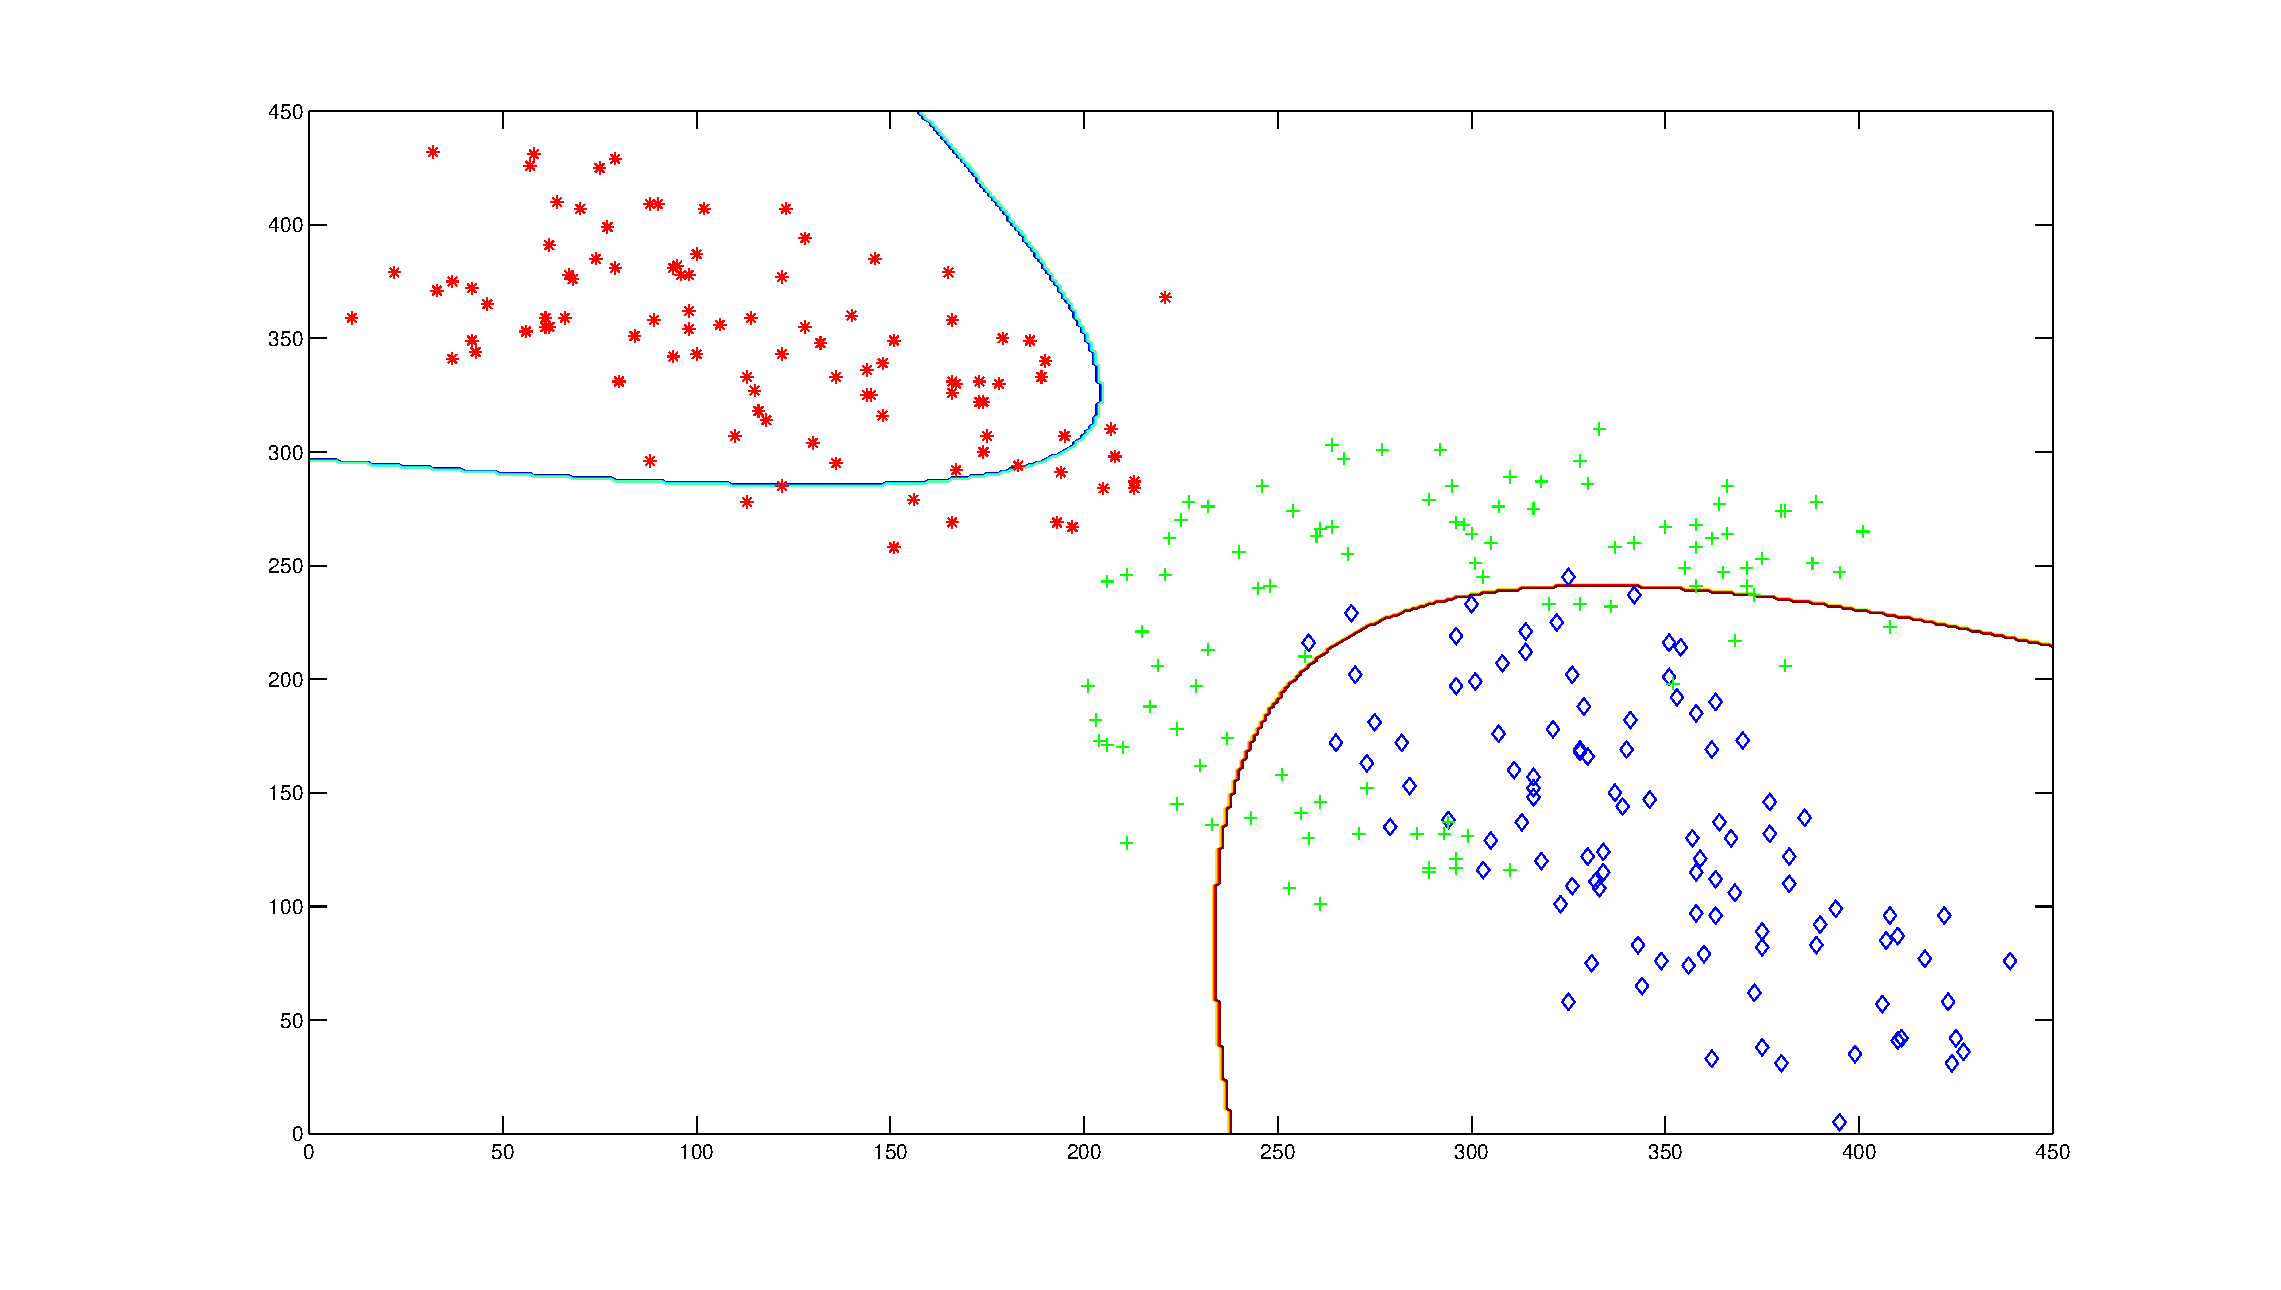
\includegraphics[scale=0.4]{twod-par}
\caption{2D Parametric Estimation}
\label{fig:twod-par}
\end{figure}

\begin{figure}
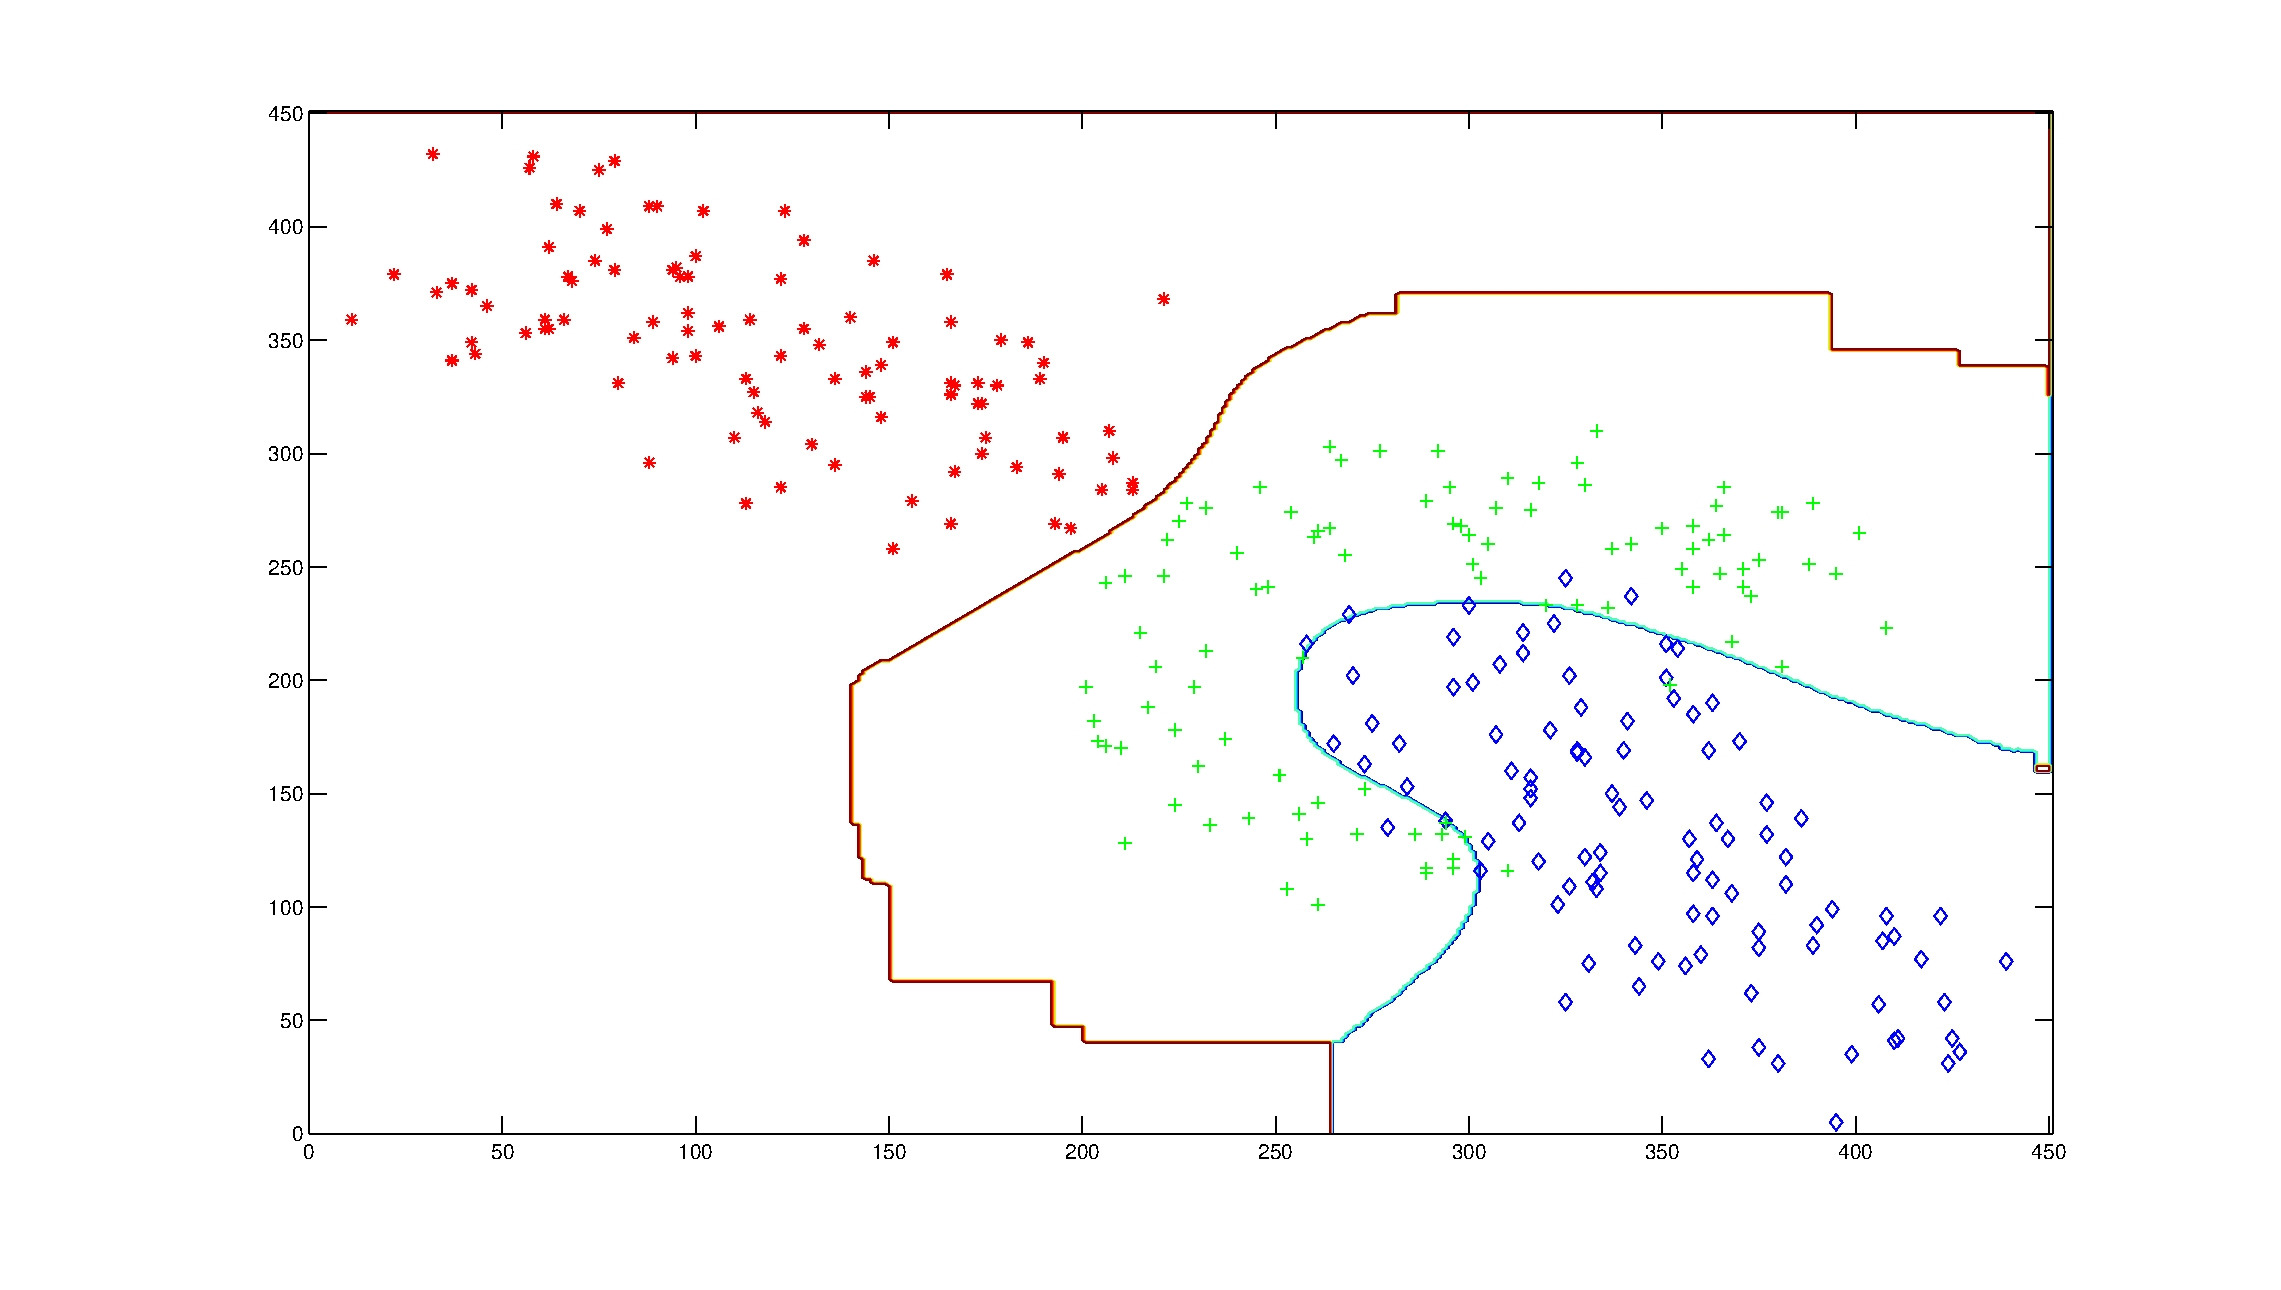
\includegraphics[scale=0.4]{twod-nonpar}
\caption{2D Non-Parametric Estimation}
\label{fig:twod-nonpar}
\end{figure}